\chapter{Cluster Membership}
\label{sec:cluster-membership}

The {\em membership} of a cluster refers to the set of daemons managed by a
common coordinator.  Cluster membership is dynamic and varies as daemons join
and leave the cluster.  The membership is split into two groups: {\em online}
daemons that actively service client requests; and {\em offline} daemons which
are known to the coordinator, but not configured to serve client requests.
Daemons may categorized as offline for a variety of reasons, including planned
maintenance, process failure, and network partitions.

This chapter describes how HyperDex manages cluster membership.
Section~\ref{sec:mem:tutorial} introduces cluster membership in the form of a
short tutorial.
Section~\ref{sec:mem:state-trans} details the state machine the coordinator uses
internally each daemon.
Finally, Section~\ref{sec:mem:commands} provides a reference-style guide to the
commands available for manually managing cluster membership.

\section{Tutorial}
\label{sec:mem:tutorial}

\section{State Transitions}
\label{sec:mem:state-trans}

\begin{description}[labelindent=\widthof{{\bf Not Available}},leftmargin=*,noitemsep,align=right]
\item[\namedlabel{srvstate:unknown}{Unknown}]
    The daemon is not known to the coordinator.  It either has not yet
    associated with the coordinator, or has been explicitly disassociated from
    the coordinator.

    Category: offline
\item[\namedlabel{srvstate:assigned}{Assigned}]
    The daemon has registered with the coordinator, but has taken no further
    action.  Once initialized, the daemon will transition from this state to
    \ref{srvstate:available}.  Daemons should only be in this state for a short
    period of time during the first time they are started.  If a daemon is in
    this state for an extended period of time, it indicates that something has
    likely gone wrong.

    Category: offline
\item[\namedlabel{srvstate:notavailable}{Not Available}]
    The daemon is in an error state where it cannot serve requests.  Daemons
    that are \ref{srvstate:notavailable} will be temporarily unmapped from the
    hyperspace until the become \ref{srvstate:available} again, at which point
    they will reintegrated into the hyperspace.  \ref{srvstate:notavailable} is
    usually a temporary condition that the daemon will rectify when it comes
    back online.  Should the daemon be permanently \ref{srvstate:notavailable},
    it may be desirable to kill and forget the daemon.

    Category: offline
\item[\namedlabel{srvstate:available}{Available}]
    The daemon is fully-operational and accepting client requests.  Daemons
    always work with the coordinator to try converging to this state in
    accordance with Figure~\ref{fig:daemon-state-machine}.

    Category: online
\item[\namedlabel{srvstate:shutdown}{Shutdown}]
    The daemon cleanly shutdown, usually in response to a \texttt{SIGINT} or
    \texttt{SIGTERM}, and the coordinator acknowledged the clean shutdown.

    Category: offline
\item[\namedlabel{srvstate:killed}{Killed}]
    The daemon was explicitly killed by the administrator.
    \ref{srvstate:killed} is permanent, and cannot be undone.  Daemons should
    self-terminate upon transitioning to \ref{srvstate:killed}.
    
    Category: offline
\end{description}

Figure~\ref{fig:daemon-state-machine} shows the state machine that the
coordinator adheres to when changing members' states.

\begin{figure}[t]
\begin{center}
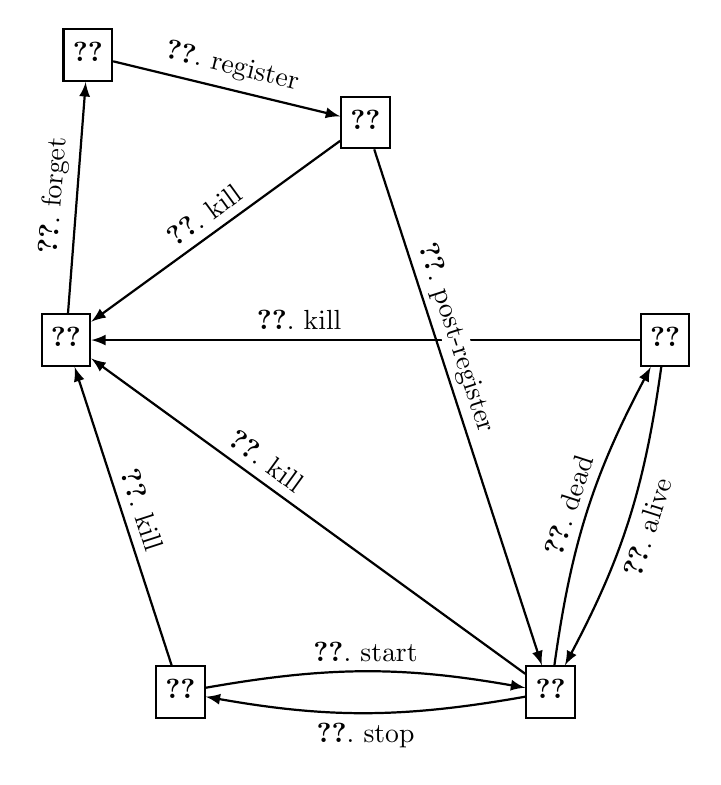
\begin{tikzpicture}
% structure things
% A at 9:30
% B at 12
% ...
% E at 7:30
\foreach \name/\angle/\text in {E/234/E, A/162/A, 
                               B/90/B, C/18/C, D/-54/D}
    \node[circle,draw=white,fill=white,text=white] (\name) at (\angle:4cm) {\text};
\node[circle,draw=white,fill=white,text=white] (F) at (126:6cm) {F};

% Place rectangles for the states
\node[rectangle,minimum height=\baselineskip,draw=black,thick] (unknown)      at (F) {\strut \ref{srvstate:unknown}};
\node[rectangle,minimum height=\baselineskip,draw=black,thick] (assigned)     at (B) {\strut \ref{srvstate:assigned}};
\node[rectangle,minimum height=\baselineskip,draw=black,thick] (notavailable) at (C) {\strut \ref{srvstate:notavailable}};
\node[rectangle,minimum height=\baselineskip,draw=black,thick] (available)    at (D) {\strut \ref{srvstate:available}};
\node[rectangle,minimum height=\baselineskip,draw=black,thick] (shutdown)     at (E) {\strut \ref{srvstate:shutdown}};
\node[rectangle,minimum height=\baselineskip,draw=black,thick] (killed)       at (A) {\strut \ref{srvstate:killed}};

% State transitions
\draw[->,>=latex,thick] (unknown) to node[midway,above,sloped] {\ref{srvtrans:reg}.~register} (assigned);
\draw[->,>=latex,thick] (killed) to node[midway,above,sloped] {\ref{srvtrans:forget}.~forget} (unknown);

\draw[->,>=latex,thick] (notavailable) edge [bend left=10] node[midway,below,sloped] {\ref{srvtrans:alive}.~alive} (available);
\draw[->,>=latex,thick] (available) edge [bend left=10] node[midway,above,sloped] {\ref{srvtrans:dead}.~dead} (notavailable);

\draw[->,>=latex,thick] (available) edge [bend left=10] node[midway,below,sloped] {\ref{srvtrans:stop}.~stop} (shutdown);
\draw[->,>=latex,thick] (shutdown) edge [bend left=10] node[midway,above,sloped] {\ref{srvtrans:start}.~start} (available);

\draw[->,>=latex,thick] (assigned) to node[midway,above,sloped] {\ref{srvtrans:kill}.~kill} (killed);
\draw[->,>=latex,thick] (notavailable) to node[midway,above,sloped,xshift=-24pt] {\ref{srvtrans:kill}.~kill} (killed);
\draw[->,>=latex,thick] (available) to node[midway,above,sloped,xshift=-24pt] {\ref{srvtrans:kill}.~kill} (killed);
\draw[->,>=latex,thick] (shutdown) to node[midway,above,sloped] {\ref{srvtrans:kill}.~kill} (killed);

\draw[->,>=latex,thick] (assigned) -- (available) node[midway,above,sloped,draw=white,fill=white,text=black,rectangle,inner sep=0pt,xshift=-24pt,yshift=2pt] {\ref{srvtrans:postreg}.~post-register};
\end{tikzpicture}
\end{center}
\caption{XXX}
\label{fig:daemon-state-machine}
\end{figure}

\begin{enumerate}[noitemsep]
\item \label{srvtrans:reg} Registration
\item \label{srvtrans:postreg} Post Registration
\item \label{srvtrans:start} Start
\item \label{srvtrans:stop} Stop
\item \label{srvtrans:alive} Alive
\item \label{srvtrans:dead} Dead
\item \label{srvtrans:kill} Kill
\item \label{srvtrans:forget} Forget
\end{enumerate}

\section{Command Reference}
\label{sec:mem:commands}
